%%%%%%%%%%%%%%%%%%%%%%%%%%%%%%%%%%%%%%%%%%%%%%%%%%%%%%%%%%%%%%%%%%%%%%%%%%%%%
%
% security.tex
%
% kalina, 17/10/2001
%
% $Id: security.tex,v 1.10 2005/11/25 13:23:43 diana Exp $
%
%%%%%%%%%%%%%%%%%%%%%%%%%%%%%%%%%%%%%%%%%%%%%%%%%%%%%%%%%%%%%%%%%%%%%%%%%%%%%


%%%%%%%%%%%%%%%%%%%%%%%%%%%%%%%%%%%%%%%%%%%%%%%%%%%%%%%%%%%%%%%%%%%%%%%%%%%%%
\chapt[chap:security]{Users, Groups, and LR Access Rights}
%%%%%%%%%%%%%%%%%%%%%%%%%%%%%%%%%%%%%%%%%%%%%%%%%%%%%%%%%%%%%%%%%%%%%%%%%%%%%

%%%% qqqqqqqqqqqqqqqqqqqqqqqqq %%%%
\begin{quote}
`Well,' he said, `it's to do with the project which first made the
software incarnation of the company profitable. It was
called Reason, and in its own way it was sensational.'

`What was it?'

`Well, it was a kind of back-to-front program. It's funny how many of
the best ideas are just an old idea back-to-front. You
see there have already been several programs written that help you to
arrive at decisions by properly ordering and analysing
all the relevant facts so that they then point naturally towards the
right decision. The drawback with these is that the decision
which all the properly ordered and analysed facts point to is not
necessarily the one you want.'

`Yeeeess ...' said Reg's voice from the kitchen.

`Well, Gordon's great insight was to design a program which allowed
you to specify in advance what decision you wished it
to reach, and only then to give it all the facts. The program's
task, which it was able to accomplish with consummate ease,
was simply to construct a plausible series of logical-sounding steps
to connect the premises with the conclusion.

`And I have to say that it worked brilliantly. Gordon was able to buy
himself a Porsche almost immediately despite being
completely broke and a hopeless driver. Even his bank manager was
unable to find fault with his reasoning. Even when
Gordon wrote it off three weeks later.'

`Heavens. And did the program sell very well?'

`No. We never sold a single copy.'

`You astonish me. It sounds like a real winner to me.'

`It was,' said Richard hesitantly. `The entire project was bought
up, lock, stock and barrel, by the Pentagon. The deal put
WayForward on a very sound financial foundation. Its moral
foundation, on the other hand, is not something I would want to
trust my weight to. I've recently been analysing a lot of the
arguments put forward in favour of the Star Wars project, and if
you know what you're looking for, the pattern of the algorithms is
very clear.

`So much so, in fact, that looking at Pentagon policies over the
last couple of years I think I can be fairly sure that the US
Navy is using version 2.00 of the program, while the Air Force
for some reason only has the beta-test version of 1.5. Odd,
that.'

{\it Dirk Gently's Holistic Detective Agency}, Douglas Adams, 1987 (pp. 55-56).
\end{quote}
%%%% qqqqqqqqqqqqqqqqqqqqqqqqq %%%%

This \chapthing\ describes the LR access mechanism which is implemented
for persistent LRs. At present there are two LR persistency storage
methods: Java serialisation and Oracle. Here we will describe their
security features in turn.

\sect{Java serialisation and LR access rights}
At present the security model is not implemented for Java
serialization. One should rely on the security control offered by
the OS in order to restrict access to certain persistent
resources.

\sect[sec:oracle_security]{Oracle Datastore and LR access rights}

{\bf Warning:} These features will not work, unless you have an
Oracle pre-installed at your site\footnote{Oracle installation is
not provided with GATE. You need to purchase this product
separately from Oracle Corp. (see \htlink{http://www.oracle.com}{
http://www.oracle.com}).} and you, or an administrator at your
site, has installed the GATE Oracle support (see
http://gate.ac.uk/gate/doc/persistence.pdf).

Oracle datastores have advanced LR access rights based on users and
groups, which are similar to those in an operating system such as Linux.

In order to be able to access an LR stored in an Oracle datastore, a
user needs to supply a user name, password and a group. These
credentials are used to determine which LRs are accessible to this user
for reading and writing.

\subsect[sec:oracle_access_modes]{Users, Groups, Sessions and Access Modes}

The security model provides primitives such as users, groups,
permissions and sessions similar to the ones provided by the
operating systems:

\begin{itemize}
    \item {\bf users} - they are identified by login name and password (each limited to 16 symbols).
    A user may be member of one or more groups.
    \item {\bf groups} - identified by name (up to 128 symbols).
    \item {\bf session} - each user must log into the datastore (by providing name, password and group) in order to use its resources.
    A session is opened when the user logs in. The default inactivity period after which the session expires and the user
    should log into the datastore again is 4 hours.
    \item {\bf access modes} -  there are four access modes in the present implementation.
    The access (Read/Write) to a resource
    according to its owner and access mode is shown in Table~\ref{table:access_modes}.
\end{itemize}

\begin{table}[htbp]
\begin{tabular} {|l|c|c|c|} \hline
Mode&Owner (R/W)& Owner's group (R/W) &Other users (R/W)\\
\cline{1-4}
%  \ &   \   & Words &Terms   \\ \cline{1-4}
World Read/ & +/+ & +/+ & +/- \\
Group Write & & & \\ \cline{1-4}
Group Read/ & +/+ & +/+ & -/- \\
Group Write & & & \\ \cline{1-4}
Group Read/ & +/+ & +/- & -/- \\
Owner Write & & & \\ \cline{1-4}
Owner Read/ & +/+ & -/- & -/- \\
Owner Write & & & \\ \cline{1-4}

\end{tabular}
\caption{Access Modes}
\label{table:access_modes}
\end{table}


When GATE is configured for use with Oracle, a superuser and group
are created:

\begin{itemize}
    \item super user - ADMIN, password  'sesame'.
    \item administrative group - ADMINS.
\end{itemize}

The superuser is similar to the root user in Unix and has access
to any resource despite its access mode.This user can also create
or remove other users We recommend that you change the password of
the superuser immediately after you have installed the Oracle
support for GATE.

\subsect[sec:oracle_user_group_admin]{User/Group Administration}

\subsubsect{Running the administration tool}

When GATE Oracle tables are first created with the database
install scripts, they only contain the {\tt ADMIN} user which is
the only user who can create and modify users and
groups.\footnote{This user is similar to the {\tt root} user in
Unix operating systems.} We do not recommend using the {\tt ADMIN}
user to store/access LRs in GATE.

Instead, immediately after installing Oracle support for GATE
datastores, some users and groups must be created by running the
{\tt UserGroupEditor} tool. Before running this tool, the URL to
the Oracle database needs to be specified in gate.xml (either the
user's own or the site-wide gate.xml). An example entry is:

<DBCONFIG
  url="jdbc:oracle:thin:GATEUSER/gate@example.dcs.shef.ac.uk:1521:gate101"
  url1="jdbc:oracle:thin:GATEUSER/gate@testdb.dcs.shef.ac.uk:1521:gate02"
/>

The example entry shows that there are two databases configured
for this site, one at each URL. There is no limit to the number of
Oracle databases one can have, but they all need to have an
attribute starting with "url", e.g., url1, url2.

To run the tool, call the gate script with the {\tt -a} parameter.

When the tool starts up, it first asks you to select which Oracle
database you wish to administer. All databases defined in the
<DBCONFIG> section of gate.xml will be shown in a listbox. Once
the database is chosen, a login dialog is shown, asking for the
user name, password and group of the {\tt ADMIN} user. The initial
password of the {\tt ADMIN} user is {\tt sesame} and the group is
{\tt ADMINS}. We advise that these are changed, the first time
this tool is run.

If all login credentials are provided correctly, the graphical tool
starts up:
%
\begin{figure}[htbp]
\begin{center}
%\epsfysize=4in
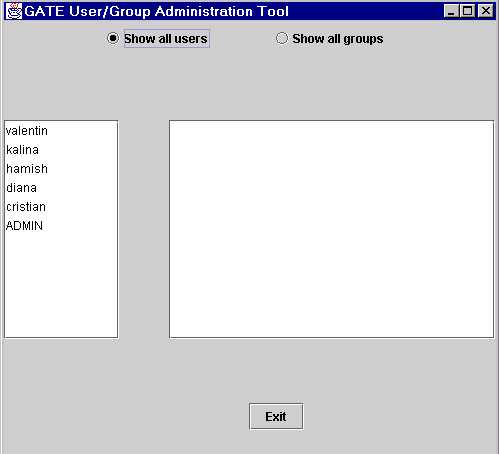
\includegraphics[scale=0.5]{user-group-tool-gui.png}
\end{center}
\caption{The User/Group Administration Tool}
\label{fig:user_group_tool_gui}
\end{figure}
%

\subsubsect{Viewing user and group information}

As shown in Figure~\ref{fig:user_group_tool_gui}, the user/group
administration tool (called the UG tool for the rest of this section)
consist of two parallel lists. By default, the left one shows a list of
all users in the database and the right one is empty.

To view the groups to which a particular user belongs, you need to
select that user in the list. Then the right list displays this user's
groups. If the list remains empty, then it means that this user does not
belong to any group.

In order to view all groups which are available, you need to switch the
tool to a {\tt Users for groups} mode, by clicking on the corresponding
radio button. This will switch the tool to showing the list of all
groups in the left panel. When you select a given group, then the right
panel shows all users who belong to that group (see
Figure~\ref{fig:user_group_tool_group_mode}).
%
\begin{figure}[htbp]
\begin{center}
%\epsfysize=4in
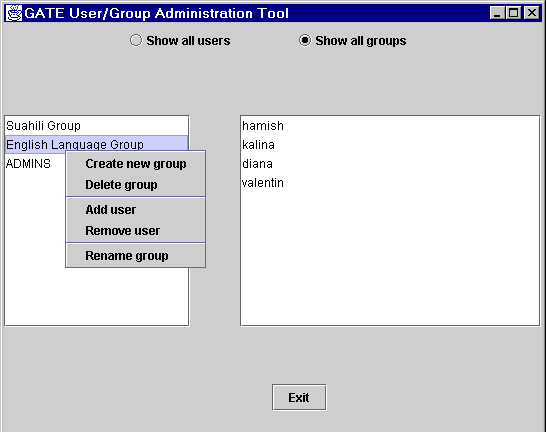
\includegraphics[scale=0.5]{user-group-tool-group-mode.png}
\end{center}
\caption{The tool in a group administration mode}
\label{fig:user_group_tool_group_mode}
\end{figure}
%

\subsubsect{User manipulation}

Users are manipulated by selecting a user in the list of users and
right-clicking on it to see the user manipulation menu. This menu
allows the following actions:
\begin{description}
        \item[Create new user:] shows a dialog where the user name and
        password of the new user must be specified.
        \item[Delete user:] delete the currently selected user.
        \item[Add to group:] shows a dialog displaying all available
        groups. Select one to add the user to it.
        \item[Remove from group:] in the given dialog, choose the group
        from which the user is to be removed.
        \item[Change password:] shows a dialog where the new password
        can be specified;
        \item[Rename user:] choose another name for the selected user.
\end{description}

All changes are automatically written to the Oracle database.

\subsubsect{Group manipulation}

Groups are manipulated by selecting a group in the list of groups and
right-clicking on it to see the group manipulation menu. This menu
allows the following actions:
\begin{description}
        \item[Create new group:] shows a dialog where the name of the
        new group must be specified.
        \item[Delete group:] delete the currently selected group.
        \item[Add user:] shows a dialog displaying all available
        users. Select one to add to the group.
        \item[Remove user:] in the given dialog, choose the user
        to be removed.
        \item[Rename group:] choose another name for the selected group.
\end{description}

All changes are automatically written to the Oracle database.

\subsect[sec:oracle_security_api]{The API}

In order to work with users and groups\footnote{See the
latest API documentation online at: \htlink{http://gate.ac.uk/gate/doc/javadoc/index.html}{http://gate.ac.uk/gate/doc/javadoc/index.html}. User and group API is
located in the {\tt gate.security} package.} programmatically, you need
to use an access controller, which is the class that provides the
connection to the Oracle database. The access controller needs to be
closed before application exit.

Once the connection is established, you need to create a session by
proving the login details of the user (user name, password and group).
Any user who can login, can use the accessor methods for users/groups,
but only the {\tt ADMIN} user has privileges to modify the data. The way
to check whether the logged in user has the right to modify data, is to
use the {\tt isPriviligedSession()} method (see below). If a mutator
method is used with a non-privileged session, a {\tt SecurityException} is
thrown. All security-related classes and all their methods are
documented in the GATE JavaDoc documentation, {\tt java.security}
package.
%
\nsmall
\begin{verbatim}

  AccessController ac = new AccessControllerImpl();
  ac.open("jdbc:oracle:thin:GATEUSER/gate@machine.ac.uk:1521:GateDB");

  Session mySession = null;
  try {
    mySession = ac.login("myUser", "myPass",ac.findGroup("myGroup").getID());
  } catch (gate.security.SecurityException ex) {
    ac.close();
    <print some error and exit>
  }

  //first check whether we have a valid session
  if (! ac.isValidSession(mySession)){
    ac.close();
    <print some error and exit>
  }

  //then check that it is an administrative session
  if (!mySession.isPrivilegedSession()) {
    ac.close();
    <print some error and exit>
  }

  User myUser = ac.findUser("myUser");
  String myName = myUser.getName()
  List myGroups = myUser.getGroups();
  ...
  <more code to access/modify groups and users here>

  //we're done now, just close the access controller connection
  ac.close();

\end{verbatim}
\nnormalsize
%
If you'd like to use a dialog, where the user can type those details,
the session can be obtained by using the {\tt login(AccessController ac,
Component parent)} static method in the {\tt UserGroupEditor} class. The
login code would then look as follows:

{\tt
  mySession = UserGroupDialog.login(ac, someParentWindow);
}

For a full example of code using the security API, see {\tt
TestSecurity.java} and {\tt UserGroupEditor.java}.
